% Copper-plate benchmark solved at T = 6 with all bounds imposed (case 6e of the
% FilterDDP evaluation). Numbers are the FilterDDP solution, which agrees with
% the independent active-set QP reference to 1.3e-9.
%
% One figure, three stacked panels, following envs/tadmm/Plotter.jl:
%
%   Panel 1 -- plot_substation_power_and_cost:
%       substation power as a black line; period cost P_Subs * c * dt on a
%       secondary axis in dark green. Demand is added as a subordinate dashed
%       line, which the Julia routine does not draw, because without it the
%       peak-shaving the battery performs is not visible.
%   Panels 2-3 -- _plot_single_battery:
%       charging P_c = -min(P_B,0) drawn POSITIVE in green, discharging
%       P_d = max(P_B,0) drawn NEGATIVE in maroon (so a bar's direction is the
%       device's action, not the sign of P_B); black zero rule; unit-width bars
%       centred at t-1/2; x from -1 to T+1/2. SOC as bars at t = 0..T with the
%       fixed initial value in indigo and the optimised values in purple, on a
%       zoomed axis so the bars run off the bottom.
%
% Per-interval quantities (P_Subs, cost, demand, P_c/P_d) are all placed at the
% interval centre t-1/2 and node quantities (B) at the nodes 0..T, so the three
% panels share one honest x-axis.
%
% Deviation: Plotter.jl reports SOC in percent of rated capacity and powers in
% kW via P_BASE; this benchmark carries neither, so everything is in p.u.
%
\definecolor{cSubs}{HTML}{000000}   % black      -- substation power
\definecolor{cCost}{HTML}{006400}   % dark green -- period cost
\definecolor{cLoad}{HTML}{31748F}   % pine       -- demand (added)
\definecolor{cChg}{HTML}{008000}    % green      -- charging    (Plots.jl :green)
\definecolor{cDis}{HTML}{800000}    % maroon     -- discharging (Plots.jl :maroon)
\definecolor{cB0}{HTML}{4B0082}     % indigo     -- fixed initial SOC
\definecolor{cSOC}{HTML}{800080}    % purple     -- optimised SOC
\definecolor{cLim}{HTML}{8C1D1D}    % maroon     -- binding limits
\definecolor{gridMajor}{HTML}{E8C4D4} % soft pink     -- major grid
\definecolor{gridMinor}{HTML}{D4D4E8} % soft lavender -- minor grid
%
\begin{figure}[!t]
\centering
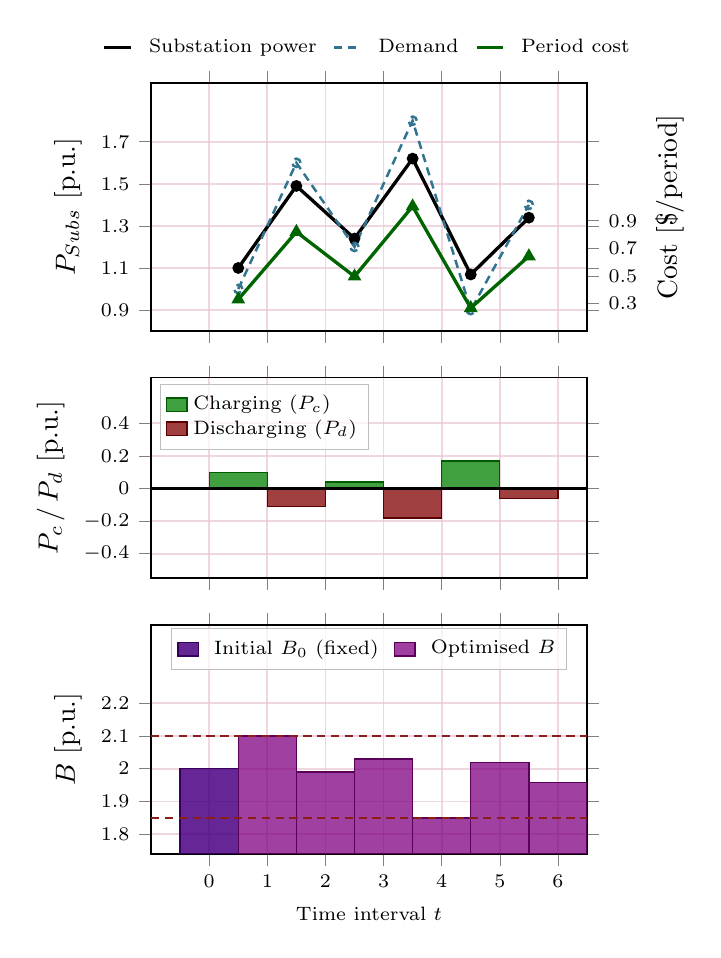
\begin{tikzpicture}
\pgfplotsset{
  every axis/.append style={
    x=21pt, scale only axis,
    xmin=-1.0, xmax=6.5,
    xtick={0,1,2,3,4,5,6},
    tick align=outside,
    tick label style={font=\scriptsize},
    label style={font=\scriptsize},
    axis line style={black, line width=0.6pt},
    grid=both,
    major grid style={line width=0.6pt, color=gridMajor, opacity=0.7},
    minor grid style={line width=0.4pt, color=gridMinor, opacity=0.6},
    legend image code/.code={\draw[#1] (0cm,-0.085cm) rectangle (0.26cm,0.085cm);},
  },
}

% ============ Panel 1: substation power, demand, period cost ============
\begin{axis}[
    name=axSub, height=0.26\columnwidth,
    ymin=0.80, ymax=1.98,
    ytick={0.9,1.1,1.3,1.5,1.7},
    yticklabel style={/pgf/number format/fixed, /pgf/number format/precision=1},
    xticklabels={},
    ylabel={$P_{\text{Subs}}$ [p.u.]}, ylabel near ticks,
    legend style={at={(0.5,1.06)}, anchor=south, legend columns=3,
                  draw=none, fill=none, column sep=0.9ex, font=\scriptsize},
    legend image code/.code={\draw[#1] (0cm,0cm) -- (0.34cm,0cm);},
]
\addplot[cSubs, line width=1.2pt, mark=*, mark size=1.5pt,
         mark options={fill=cSubs, draw=cSubs}]
  coordinates {(0.5,1.100000) (1.5,1.490000) (2.5,1.240000)
               (3.5,1.620000) (4.5,1.069048) (5.5,1.339048)};
\addlegendentry{Substation power}
\addplot[cLoad, densely dashed, line width=0.9pt, mark=o, mark size=1.5pt,
         mark options={draw=cLoad}]
  coordinates {(0.5,1.0) (1.5,1.6) (2.5,1.2) (3.5,1.8) (4.5,0.9) (5.5,1.4)};
\addlegendentry{Demand}
\addlegendimage{cCost, line width=1.2pt, mark=triangle*, mark size=1.7pt,
                mark options={fill=cCost, draw=cCost}}
\addlegendentry{Period cost}
\end{axis}

% right axis of panel 1: period cost
\begin{axis}[
    at={(axSub.south west)}, anchor=south west, height=0.26\columnwidth,
    % offset, as in input_curves_fig.tex: cost tracks substation power closely
    % and would otherwise overplot it
    ymin=0.10, ymax=1.90,
    xtick=\empty, ytick={0.3,0.5,0.7,0.9},
    scaled y ticks=false,
    yticklabel style={/pgf/number format/fixed, /pgf/number format/precision=1},
    ylabel={Cost [\$/period]}, ylabel near ticks,
    axis x line=none, axis y line*=right, grid=none,
]
\addplot[cCost, line width=1.2pt, mark=triangle*, mark size=1.7pt,
         mark options={fill=cCost, draw=cCost}]
  coordinates {(0.5,0.330000) (1.5,0.819500) (2.5,0.496000)
               (3.5,1.004400) (4.5,0.267262) (5.5,0.642743)};
\end{axis}

% ============ Panel 2: charging / discharging ============
\begin{axis}[
    name=axPow, at={(axSub.below south west)}, anchor=north west,
    yshift=-2.0mm, height=0.21\columnwidth,
    ymin=-0.55, ymax=0.68,
    ytick={-0.4,-0.2,0,0.2,0.4},
    yticklabel style={/pgf/number format/fixed, /pgf/number format/precision=1},
    xticklabels={},
    ylabel={$P_c\,/\,P_d$ [p.u.]}, ylabel near ticks,
    legend style={at={(0.02,0.97)}, anchor=north west, draw=black!25,
                  fill=white, fill opacity=0.7, text opacity=1,
                  font=\scriptsize, row sep=-2pt, inner sep=2pt},
    legend cell align=left,
]
\addplot[ybar, bar width=21pt, draw=cChg!70!black, fill=cChg, fill opacity=0.75,
         line width=0.5pt]
  coordinates {(0.5,0.100000) (1.5,0.0) (2.5,0.040000)
               (3.5,0.0) (4.5,0.169048) (5.5,0.0)};
\addlegendentry{Charging ($P_c$)}
\addplot[ybar, bar width=21pt, draw=cDis!70!black, fill=cDis, fill opacity=0.75,
         line width=0.5pt]
  coordinates {(0.5,0.0) (1.5,-0.110000) (2.5,0.0)
               (3.5,-0.180000) (4.5,0.0) (5.5,-0.060952)};
\addlegendentry{Discharging ($P_d$)}
\addplot[black, line width=1.0pt, forget plot, domain=-1.0:6.5, samples=2] {0};
\end{axis}

% ============ Panel 3: state of charge ============
\begin{axis}[
    at={(axPow.below south west)}, anchor=north west,
    yshift=-2.0mm, height=0.24\columnwidth,
    ymin=1.74, ymax=2.44,
    ytick={1.8,1.9,2.0,2.1,2.2},
    yticklabel style={/pgf/number format/fixed, /pgf/number format/precision=1},
    xlabel={Time interval $t$},
    ylabel={$B$ [p.u.]}, ylabel near ticks,
    legend style={at={(0.5,0.985)}, anchor=north, legend columns=2,
                  draw=black!25, fill=white, fill opacity=0.7, text opacity=1,
                  font=\scriptsize, column sep=0.8ex, inner sep=2pt},
    legend cell align=left,
]
\addplot[ybar, bar width=21pt, draw=cB0!70!black, fill=cB0, fill opacity=0.85,
         line width=0.5pt]
  coordinates {(0,2.000000)};
\addlegendentry{Initial $B_0$ (fixed)}
\addplot[ybar, bar width=21pt, draw=cSOC!70!black, fill=cSOC, fill opacity=0.75,
         line width=0.5pt]
  coordinates {(1,2.100000) (2,1.990000) (3,2.030000)
               (4,1.850000) (5,2.019048) (6,1.958095)};
\addlegendentry{Optimised $B$}
\addplot[cLim, densely dashed, line width=0.9pt, forget plot,
         domain=-1.0:6.5, samples=2] {2.10};
\addplot[cLim, densely dashed, line width=0.9pt, forget plot,
         domain=-1.0:6.5, samples=2] {1.85};
\end{axis}
\end{tikzpicture}
\caption{The benchmark solved at $T = 6$ with all bounds
\eqref{eq:cp_pg_lim}--\eqref{eq:cp_soc_lim} imposed.  Battery actions use the
convention of the tADMM study: charging is drawn upward in green and
discharging downward in maroon, so a bar's direction reads as the device's
action rather than as the sign of $P_B^t$.  Read it as one worked example.  The
battery charges in the cheap intervals $t = 1, 3, 5$ and discharges into the
expensive ones $t = 2, 4, 6$, which is why the substation trace in the top panel
is visibly flatter than the demand it serves --- it is pulled down at the two
demand peaks and pushed up in the trough at $t = 5$, where energy is cheapest.
Substation import is unlimited above, so the schedule is bounded only by the
device: stored energy is pushed onto $B^{\max} = 2.10$ after the first charge
and drawn right down onto $B^{\min} = 1.85$ after the interval-$4$ discharge
(dashed rules in the lower panel).  Those two limits are exactly the active set
the independent reference solver reports, and the trajectory sits on them to
$1.2 \times 10^{-9}$.  The battery power bounds, $-0.5 \leq P_B^t \leq 0.30$,
never bind.}
\label{fig:schedule}
\end{figure}
